% pgf-interference package: English manual
% Version 0.1
% 9. Januar 2022
\documentclass{scrartcl}
\usepackage[UKenglish]{babel}
\usepackage{pgf-interference}
\usepackage{libertinus}
\usepackage{cnltx-example}
\usepackage{mathtools}
\usepackage{pgfplots}
\usepackage{worldflags}
\usepackage[locale=UK,mode=match]{siunitx}
\usepackage[colorlinks=true,
  allcolors=black,
  bookmarksopen=true,
  bookmarksopenlevel=0,
  bookmarksnumbered=true,
  pdfencoding=auto,
  pdftitle={Drawing interference patterns with pgf/TikZ},
  pdfsubject={Manual for the pgf-interference package},
  pdfkeywords={latex pgf tikz interference},
  pdfauthor={K. Wehr}]{hyperref}

\definecolor{pgfinterferencered}{wave}{632.8}

\definecolorscheme{pgfinterferencecolorscheme}{cs => cnltxformalblue,
  option => cnltxgreen,
  cnltx => pgfinterferencered}

\setcnltx{add-cmds = {pgfinterferenceoptions,pgfinterferencepattern},
  color-scheme = pgfinterferencecolorscheme,
  add-listings-options = {numbers=none},
  pre-output = {\raggedright}}

\makeatletter
\setlength{\cnltx@before@skip}{5pt plus1pt minus1pt}
\setlength{\cnltx@after@skip}{1pt plus1pt minus1pt}
\makeatother

\selectcolormodel{rgb}

\setmonofont{DejaVu Sans Mono}[Scale=MatchLowercase]

\pgfplotsset{compat=newest}
\usetikzlibrary{angles}

\newenvironment{Befehlsliste}{\begin{list}{}{
  \setlength\leftmargin{0pt}
  \setlength\itemindent{-1em}
  \setlength\parsep{0pt}
  \setlength\listparindent{\parindent}
  \setlength\itemsep{\topsep}}}{\end{list}}

\newcommand*\Befehlsbeschreibung[2]{\item\cs{#1}#2\\}

\newcommand*\Optionsbeschreibung[3]{\item\choicekey{#1}{#2}
  \hfill Default:~\code{#3}\\}

\newcommand*\OptionsbeschreibungZahl[2]{\item
  \choicekey{#1}{\meta{number}}
  \hfill Default:~\code{#2}\\}

\newcommand*\Paket[1]{\textsf{#1}}
\newcommand\inter{\textcolor{pgfinterferencered}{\Paket{pgf-interference}}}
\newcommand\pgftikz{\Paket{\textsc{pgf}/Ti\textit{k}Z}}
\newcommand\pakettikz{\Paket{Ti\textit{k}Z}}
\newcommand\AutorNachname{Wehr}
\newcommand\AutorVorname{Keno}

\begin{document}

\begin{center}
\fontsize{41}{41}\selectfont\textsc{\inter}

\medskip
\pgfinterferencepattern{}

\LARGE
\rmfamily
Drawing interference patterns with \pgftikz

\bigskip
\Large
\textcolor{pgfinterferencered}{Version 0.1}

\medskip
\large
\today

\bigskip
\textit{Package author}

\smallskip
\AutorVorname\ \AutorNachname

\bigskip
\textit{Questions and bug reports}

\smallskip
\normalsize
\url{https://codeberg.org/wehr/pgf-interference}
\end{center}

\begin{abstract}
\noindent This \LaTeX\ package makes it possible to simulate interference patterns occuring on a screen if monochromatic light is diffracted at regular structures of slits. It makes use of the \pgftikz\ graphics package.

\medskip
\noindent The package is still in an experimental stage. The user interface may change in future versions.

\medskip
\noindent
\worldflag[width=9pt,framewidth=0pt]{DE} A German version of this manual is available in the file \texttt{pgf-interference-de.pdf}.
\end{abstract}

\vfill
\tableofcontents

\newpage
\section{Introduction}
The occurence of interference patterns after passing through fine structures of slits gives impressive evidence for the wave nature of light. Such interference patterns are already examined in physics lessons in upper secondary school.

As only a limited stock of light sources and diffraction objects is available in physics collections, it is desirable to be able to present the interference images for wavelengths and slit dimensions that are not experimentally accessible.
\begin{center}
\pgfinterferencepattern{wavelength=450e-9}

\small
Interference pattern for light with a wavelength of
\qty{450}{nm}
behind a double slit

\medskip
\pgfinterferencepattern{wavelength=550e-9,slits=4,intensity=3}

\small
Interference pattern for light with a wavelength of
\qty{550}{nm}
behind a quadruple slit

\medskip
\pgfinterferencepattern{slits=1,slit-width=5e-5,intensity=10}

\small
Interference pattern for light with a wavelength of
\qty{633}{nm}
behind a single slit
\end{center}

The \inter\ package makes this possible. Only monochromatic light and regular slit structures (single, double, and multiple slits) are supported. Also, so far only interference fringes can be displayed, as they occur when the light is expanded vertically, not the typical “interference dots” generated by a laser beam.

The package is subject to the
\emph{\LaTeX\ Project Public License},
version 1.3 or later.%
\footnote{\url{http://www.latex-project.org/lppl.txt}}

\newpage
\section{Usage}
The package is loaded as usual:
\begin{sourcecode}
  \usepackage{pgf-interference}
\end{sourcecode}
This also loads the \pakettikz{} package indirectly.

Compiling documents with many interference patterns can take a long time due to the calculations involved. Therefore, there is a draft mode in which only the screen is drawn, but no interference pattern, which is much faster. The draft mode is activated by the package option
\code{draft}.
\begin{sourcecode}
  \usepackage[draft]{pgf-interference}
\end{sourcecode}

The \inter{} package defines two commands:
\begin{Befehlsliste}
\Befehlsbeschreibung{pgfinterferencepattern}{\marg{options}}
Generates an interference pattern. The argument is a comma-separated list of options. The available options are described in section \ref{Optionen}.
\begin{example}
  \pgfinterferencepattern{slits=3,wavelength=590e-9,slit-distance=3e-5,intensity=2}
\end{example}
\Befehlsbeschreibung{pgfinterferenceoptions}{\marg{options}}
Sets options without drawing an interference pattern.
\begin{sourcecode}
  \pgfinterferenceoptions{slit-width=1e-6,screen-distance=3.5,screen-width=0.15}
\end{sourcecode}
\end{Befehlsliste}

\newpage
\section{Options\label{Optionen}}
\pgfinterferenceoptions{screen-width=0.05,screen-height=0.015}
All lengths of the experiment such as the wavelength, the slit distance, the screen width, etc.\@ are to be given in metres, possibly using the scientific notation. For example, a slit distance of
\qty{0,1}{mm}
can be typed in as
\code{0.0001}, \code{0.1e-3}, or  \code{1e-4}.\footnote{The lengths are internally treated as floating point numbers of the \Paket{expl3} module \Paket{l3fp}, whose syntax therefore also applies to the input.}

\subsection{Options for the light}
\begin{Befehlsliste}
\OptionsbeschreibungZahl{wavelength}{632.8e-9}
Wavelength of the light in \unit{m}. The default setting corresponds to the wavelength of the helium-neon laser
(\qty{632,8}{nm}).
The wavelength does not only influence the position but also the colour of the interference maxima, which is determined with the help of the \Paket{xcolor} package.

For wavelengths outside the visible range, the maxima are shown in black.\footnote{According to the algorithm of the \Paket{xcolor} package, this is the case for wavelengths below
\qty{363}{nm}
and above
\qty{814}{nm}.}
In order to make such maxima visible, the screen colour should be set to white. The longest possible wavelength is
\qty{1}{m}.
\begin{sidebyside}
  \pgfinterferencepattern{wavelength=590e-9}
  \pgfinterferencepattern{wavelength=350e-9,screen-color=white}
\end{sidebyside}
\OptionsbeschreibungZahl{intensity}{1.0}
Relative intensity of the light. If not all expected maxima are visible, the value should be increased.
\begin{sidebyside}
  \pgfinterferencepattern{slits=5}
  \pgfinterferencepattern{slits=5,intensity=6.5}
\end{sidebyside}
\end{Befehlsliste}

\subsection{Options for the diffraction object}
\begin{Befehlsliste}
\OptionsbeschreibungZahl{slits}{2}
Number of slits
\begin{sidebyside}
  \pgfinterferencepattern{slits=3}
  \pgfinterferencepattern{slits=20}
\end{sidebyside}
\OptionsbeschreibungZahl{slit-distance}{1e-4}
Slit distance in m
\begin{sidebyside}
  \pgfinterferencepattern{slit-distance=2e-4}
  \pgfinterferencepattern{slit-distance=5e-5}
\end{sidebyside}
\OptionsbeschreibungZahl{slit-width}{1e-5}
Slit width in m
\begin{sidebyside}
  \pgfinterferencepattern{slit-width=2e-5}
  \pgfinterferencepattern{slit-width=3.5e-5}
\end{sidebyside}
\end{Befehlsliste}

\subsection{Options for the screen}
\begin{Befehlsliste}
\OptionsbeschreibungZahl{screen-distance}{1.0}
Distance of the screen from the diffraction object in m
\begin{sidebyside}
  \pgfinterferencepattern{screen-distance=0.8}
  \pgfinterferencepattern{screen-distance=1.6}
\end{sidebyside}
\OptionsbeschreibungZahl{screen-width}{0.1}
Width of the screen in m
\OptionsbeschreibungZahl{screen-height}{0.03}
Height of the screen in m
\OptionsbeschreibungZahl{scale}{1.0}
Factor by which the screen is scaled in the figure

The dimensions for width and height refer to the real screen. The size of the screen in the figure depends on the value of the \option{scale} option.
\begin{sidebyside}
  \pgfinterferencepattern{screen-width=0.06,screen-height=0.01}
  \pgfinterferencepattern{slits=10,slit-distance=2e-6,slit-width=2e-7,screen-width=2,screen-height=0.5,scale=0.03}
\end{sidebyside}
\Optionsbeschreibung{screen-color}{\meta{colour}}{black}
Colour of the screen. The syntax of the \Paket{xcolor} package applies.
\begin{sidebyside}
  \pgfinterferencepattern{screen-color=yellow}
  \pgfinterferencepattern{screen-color=green!25!black}
\end{sidebyside}
\Optionsbeschreibung{ruler}{above,below,screen,none}{none}
A ruler with a centimetre scale can be displayed above or below the screen.

With \code{ruler=screen}, the ruler itself serves as a screen. In this case the \option{screen-height} and \option{screen-color} options are ignored.
\begin{example}
  \pgfinterferenceoptions{screen-width=0.135,screen-height=0.025}
  \pgfinterferencepattern{ruler=above}
  \pgfinterferencepattern{ruler=below,scale=0.8}
  \pgfinterferencepattern{ruler=screen}
\end{example}
\end{Befehlsliste}

\section{Physical theory}
The textbooks (e.\,g. \cite{BS}, p. 373) give the following formula for the intensity of the light diffracted in the direction of $\varphi$ behind a multiple slit:
\begin{equation}
I(\varphi)\sim\frac{\sin^2\bigl(\frac{\pi\,b}{\lambda}\,\sin\varphi\bigr)}{\bigl(\frac{\pi\,b}{\lambda}\,\sin\varphi\bigr)^2}\cdot\frac{\sin^2\bigl(\frac{p\,\pi}{\lambda}\,s\,\sin\varphi\bigr)}{\sin^2\bigl(\frac{\pi}{\lambda}\,s\,\sin\varphi\bigr)}\label{Winkelabhaengigkeit}
\end{equation}
where $b$ is the slit width, $s$ the slit distance, and $p$ the number of slits.

The first factor describes the intensity distribution as a result of diffraction at the single slit, the second the interference at an ideal multiple slit (see Fig.\@
\ref{Intensitaetsverteilung}).
\begin{figure}
\centering
\begin{minipage}{13,4cm}
\raggedleft
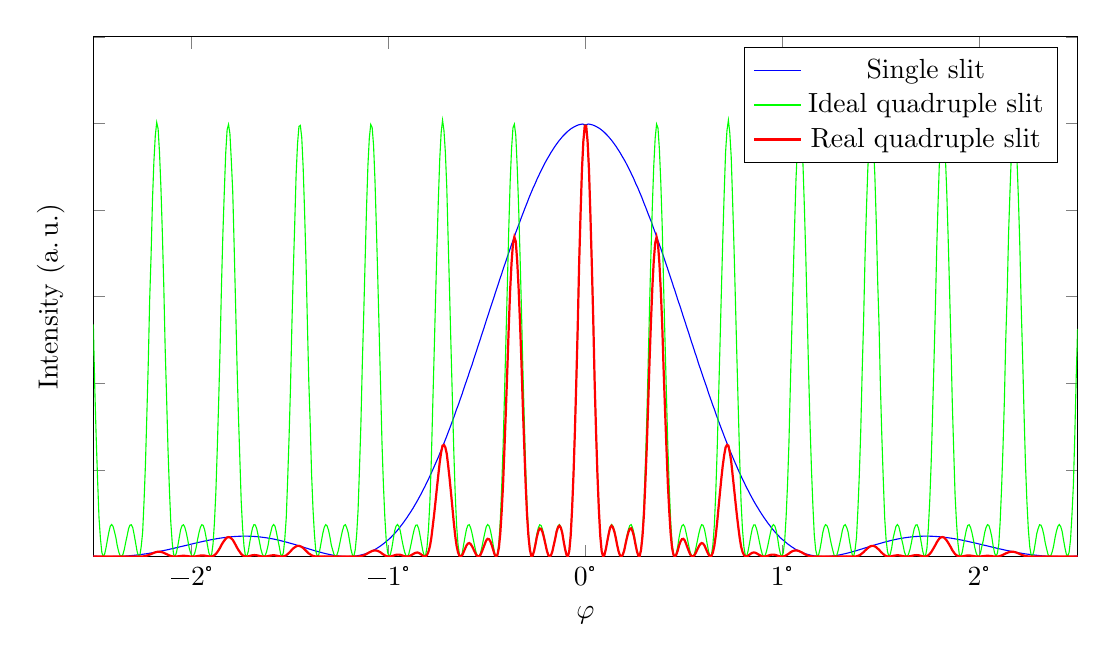
\begin{tikzpicture}
\begin{axis}[xmin=-2.5,xmax=2.5,ymin=0,ymax=1.2,xlabel=$\varphi$,ylabel=Intensity (a.\,u.),xtick={-2,...,2},xticklabels={\ang{-2},\ang{-1},\ang{0},\ang{1},\ang{2}},yticklabels=\empty,x=2.5cm,y=5.5cm]
\addplot[domain=-2.5:2.5,samples=500,blue] {(sin(180*3e-5/632.8e-9*sin(x)))^2/(pi*3e-5/632.8e-9*sin(x))^2};
\addplot[domain=-2.5:2.5,samples=700,green] {(sin(4*180/632.8e-9*1e-4*sin(x)))^2/(sin(180/632.8e-9*1e-4*sin(x)))^2/16};
\addplot[domain=-2.5:2.5,samples=700,thick,red] {(sin(180*3e-5/632.8e-9*sin(x)))^2/(pi*3e-5/632.8e-9*sin(x))^2*(sin(4*180/632.8e-9*1e-4*sin(x)))^2/(sin(180/632.8e-9*1e-4*sin(x)))^2/16};
\legend{Single slit, Ideal quadruple slit, Real quadruple slit}
\end{axis}
\end{tikzpicture}

\medskip
\pgfinterferencepattern{slits=4,slit-width=3e-5,screen-distance=1.431,screen-width=0.125,screen-height=0.025,intensity=6}
\end{minipage}
\caption{Intensity distribution and interference pattern for a quadruple slit with a slit distance of
\qty{0,1}{mm}
and a slit width of
\qty{30}{\micro\m}
at a wavelength of
\qty{632,8}{nm}\label{Intensitaetsverteilung}}
\end{figure}

\begin{figure}
\centering
\begin{tikzpicture}[font=\small]
\draw[thick] (-3,5)--node[above] {Screen} (3,5);
\draw (0,0) coordinate (O)--node[left] {$a$} (0,5) coordinate(A);
\draw (0,0)--node[right] {$e$} (2,5) coordinate (B);
\draw[dotted,thick] (-2,0)--node[below] {Diffraction object} (2,0);
\path (A)--node[below] {$x$} (B);
\draw pic[draw,angle radius=1.4cm,pic text={$\varphi$}] {angle=B--O--A};
\end{tikzpicture}
\caption{Relationship between the diffraction angle
$\varphi$
and the position
$x$
on the screen
\label{Dreieck}}
\end{figure}
To display the interference pattern, we need the intensity as a function of the position $x$ on the screen. From Fig.\@ 2 we get
\begin{equation}
\sin\varphi=\frac{x}{e}=\frac{x}{\sqrt{a^2+x^2}}\label{Sinus}
\end{equation}
where $a$ is the screen distance. Substituting
\eqref{Sinus}
into
\eqref{Winkelabhaengigkeit}
gives:
\[I(x)\sim\frac{\sin^2\left(\frac{\pi\,b\,x}{\lambda\,\sqrt{a^2+x^2}}\right)}{\left(\frac{\pi\,b\,x}{\lambda\,\sqrt{a^2+x^2}}\right)^2}\cdot\frac{\sin^2\left(\frac{p\,\pi\,s\,x}{\lambda\,\sqrt{a^2+x^2}}\right)}{\sin^2\left(\frac{\pi\,s\,x}{\lambda\,\sqrt{a^2+x^2}}\right)}\]
The calculation of the interference patterns is based on this formula.

The reduction of the intensity due to the increasing distance from the diffraction object with increasing $x$ is not taken into account.

\begin{thebibliography}{9}
\bibitem{BS} Bergmann/Schaefer: Lehrbuch der Experimentalphysik. Band 3: Optik, hrsg. von Heinrich Gobrecht, \textsuperscript{7}1978.
\end{thebibliography}

\end{document}
